\documentclass[11pt]{article}

\usepackage{tikz}
\usepackage{circuitikz}
\usepackage{amsmath}
\usepackage{amssymb}
\usepackage{float}
\DeclareMathOperator{\Tr}{Tr}

\usepackage{color}
\usepackage{listings}
\usepackage{setspace}
\definecolor{Code}{rgb}{0,0,0}
\definecolor{Decorators}{rgb}{0.5,0.5,0.5}
\definecolor{Numbers}{rgb}{0.5,0,0}
\definecolor{MatchingBrackets}{rgb}{0.25,0.5,0.5}
\definecolor{Keywords}{rgb}{0,0,1}
\definecolor{self}{rgb}{0,0,0}
\definecolor{Strings}{rgb}{0,0.63,0}
\definecolor{Comments}{rgb}{0,0.63,1}
\definecolor{Backquotes}{rgb}{0,0,0}
\definecolor{Classname}{rgb}{0,0,0}
\definecolor{FunctionName}{rgb}{0,0,0}
\definecolor{Operators}{rgb}{0,0,0}
\definecolor{Background}{rgb}{0.98,0.98,0.98}
\lstdefinelanguage{Python}{
numbers=left,
numberstyle=\footnotesize,
numbersep=1em,
xleftmargin=1em,
framextopmargin=2em,
framexbottommargin=2em,
showspaces=false,
showtabs=false,
showstringspaces=false,
frame=l,
tabsize=4,
% Basic
basicstyle=\ttfamily\small\setstretch{1},
backgroundcolor=\color{Background},
% Comments
commentstyle=\color{Comments}\slshape,
% Strings
stringstyle=\color{Strings},
morecomment=[s][\color{Strings}]{"""}{"""},
morecomment=[s][\color{Strings}]{'''}{'''},
% keywords
morekeywords={import,from,class,def,for,while,if,is,in,elif,else,not,and,or,print,break,continue,return,True,False,None,access,as,,del,except,exec,finally,global,import,lambda,pass,print,raise,try,assert},
keywordstyle={\color{Keywords}\bfseries},
% additional keywords
morekeywords={[2]@invariant,pylab,numpy,np,scipy},
keywordstyle={[2]\color{Decorators}\slshape},
emph={self},
emphstyle={\color{self}\slshape},
%
}
\linespread{1.3}

\title{Research Summary}
\author{Cesar Eduardo Garza}

\begin{document}
\maketitle

In our research into Topological Electronic Lattices, we have looked into RLC circuits with the following layout:

\begin{figure}[h!]
	\begin{center}
		\begin{circuitikz}
			\draw (0,0)
			to[R=$-R$] (0, 2)
			to[short] (2, 2)
			to[C=$C$] (2, 0)
			to[short] (0, 0);
			\draw(2, 0)
			to[short](4, 0)
			to[american inductor=$L$] (4, 2)
			to[short] (2, 2)
			to[short] node[ground] {} (2, 0);
			\draw (2, 0)
			to[short] node[draw, circle, fill=white, minimum size = 10pt] {$V_1$} (2,3);
			\draw (0,2)
			to[short](-2, 2);
			\draw (4, 2)
			to[C=$C_c$] (6,2)
			to[american inductor=$L$] (6,0)
			to[short] (8,0)
			to[C=$C$] (8, 2)
			to[short] (6,2);
			\draw (8, 0)
			to[short] (10,0)
			to[R=$R$] (10, 2)
			to[short] (8, 2)
			to[short] node[draw, circle, fill=white, minimum size = 10pt]{$V_2$} (8,3);
			\draw(8,0)
			to[short] node[ground] {} (8,0);
			\draw(10,2)
			to[short] (12,2);
		\end{circuitikz}
	\end{center}
	\caption{The basic circuit schematic}
\end{figure}

The two loops separated by the Capacitor $C_c$ will henceforth be referred to as "subcircuits". We then applied Kirchhoff's current and voltage laws to obtain the following matrix:
\[
\begin{pmatrix}
{-i \gamma + \frac{1}{\omega} - \omega (1+\kappa)} & {\omega \kappa} \\
{\omega \kappa} & {i \gamma + \frac{1}{\omega} - \omega (1 + \kappa)}
\end{pmatrix}
\begin{pmatrix}
V_1 \\
V_2
\end{pmatrix} = 0
\]
where $\kappa = \frac{C_c}{C}$, $\gamma = \frac{1}{R} \sqrt{\frac{L}{C}}$, and $\omega = \omega' \sqrt{LC}$

We then coupled an arbitrary amount of these circuits using a capacitor $C_k$ as shown below:

\begin{figure}[h!]
	\begin{center}
		\begin{circuitikz}
			\draw(0,0)
			to[american inductor = $L$] (0, 2)
			to[short] (2, 2)
			to[C = $C$] (2, 0)
			to[short] (0, 0);
			\draw(0, 2)
			to[C = $C_c$] (-2, 2);
			\draw (2, 2)
			to[short] node[draw, circle, fill=white, minimum size = 10pt]{$V_2$} (2, 3);
			\draw (2, 2)
			to[short] (4, 2)
			to[R = $R$] (4, 0)
			to[short] node[ground] {} (2, 0);
			\draw (4, 2)
			to[C=$C_k$] (6,2)
			to[R=$-R$] (6, 0)
			to[short] node[ground] {} (8, 0)
			to[C=$C$] (8, 2)
			to[short] (6, 2);
			\draw (8,2)
			to[short] node[draw, circle, fill=white, minimum size=10pt]{$V_3$} (8,3);
			\draw (8,2)
			to[short] (10,2)
			to[american inductor=$L$] (10, 0)
			to[short] (8,0);
			\draw(10,2)
			to[C=$C_c$] (12,2);
		\end{circuitikz}
	\end{center}
	\caption{Coupling between two sets of circuits}
\end{figure}

This coupling gave us the following system of equations by following Kirchhoff's Current and Voltage laws for the case of two circuits linked together:

\begin{subequations}
	\begin{align*}
		-\frac{V_1}{R}+i\omega'CV_1+\frac{V_1}{i\omega'L}+i\omega'C_c(V_1-V_2)&  &= 0 \\
		\frac{V_2}{R}+i\omega'CV_2+\frac{V_2}{i\omega'L}-i\omega'C_c(V_1-V_2)&+i\omega'C_k(V_2-V_3) &= 0 \\
		-\frac{V_3}{R}+i\omega'CV_3+\frac{V_3}{i\omega'L}+i\omega'C_c(V_3-V_4)&-i\omega'C_k(V_2-V_3) &=0 \\
		\frac{V_4}{R}+i\omega'CV_4+\frac{V_4}{i\omega'L}-i\omega'C_c(V_3-V_4)& &=0
	\end{align*}
\end{subequations}

This coupling follows a very simple pattern, which can be generalized quite easily to an arbitrary number of circuits coupled together, which led to the following in matrix form after the systems of equations is multiplied by the impedance of the circuit $\sqrt{\frac{L}{C}}$:
\[
\begin{pmatrix}
a^{*} & b & 0 & 0 & \dots & 0\\
b & d & c & 0 & \dots & 0\\
0 & c & d^{*} & b & \dots & 0\\
0 & 0 & b & d & \dots & 0\\
\vdots & \ddots & \ddots & \ddots & \ddots & \vdots\\
0 & 0 & 0 & \dots & b & a
\end{pmatrix}
\begin{pmatrix}
V_1\\
V_2\\
V_3\\
V_4\\
\vdots\\
V_{2n}
\end{pmatrix} = 0
\]
Where $a = i \gamma + \frac{1}{\omega} - \omega (1 + \kappa)$, $b=\omega \kappa$, $c = \omega \kappa'$, $d = i \gamma + \frac{1}{\omega} - \omega (1 + \kappa + \kappa')$, $\kappa' = \frac{C_k}{C}$, and $x^{*}$ refers to the complex conjugate of $x$.
\\
\\
If we refer to the matrix as $A$, then it is easy to see that $A^T = A$, and the matrix is symmetric. Additionally, it is easy to see that $\Tr{(A)} \in \mathbb{R}$ which, while it is not definitive proof, is a strong indication that eigenvalues of $A$ will be found in complex conjugate pairs.
\\
\\
To evaluate the eigenvalues of $A$ symbolically, sympy was used. The following is the code used to generate the matrices for 4 circuits coupled together:

\begin{lstlisting}[language=Python]
from sympy import *
init_printing(use_unicode = True)

w, k, kappa, g = symbols("w k k' g")


a, b, c, d = symbols('a b c d')
firstLine = [-I*g+1/w-w*(1+k),w*k]
evenLine = [w*k, I*g+1/w-w*(1+k+kappa), w*kappa]
oddLine = [w*kappa, -I*g+1/w-w*(1+k+kappa), w*k]
lastLine = [w*k, I*g+1/w-w*(1+k)]


def generateMatrix(size):
    mat = []
    mat.append([*firstLine, *[0]*2*(size-1)])
    for i in range((size - 1) * 2):
        if i % 2 is 0:
            mat.append([*[0]*i, *evenLine, *[0]*(2*(size-1)-i - 1)])
        else:
            mat.append([*[0]*i, *oddLine, *[0]*(2*(size - 1) - i - 1)])
    mat.append([*[0]*2*(size - 1), *lastLine])
    return Matrix(mat)
 
fourCase = generateMatrix(4)
fourEigen = fourCase.eigenvals()
pprint(simplify(fourEigen))
\end{lstlisting}

From running the above code on cases for $n=2,3,4,5,6$, we determined that eigenvalues follow the following order:
First, due to $A$ being tridiagonal, there will always be the two trivial eigenvalues that follow for all couplings of the circuits, even for $n=1$:
\[
\lambda = -\omega (1+\kappa) + \frac{1}{\omega} \pm \sqrt{-\gamma^2 +\omega^2 \kappa^2}
\]
For cases $n > 1$, there are the following additional eigenvalues:
\[
\lambda = -\omega (1+\kappa + \kappa') + \frac{1}{\omega} \pm \sqrt{-\gamma^2 + \omega^2 (\kappa^2 + \lambda' \kappa \kappa' + \kappa'^2)}
\]
where $\lambda'$ is an as-of-yet undetermined variable. Using the code above, we determined the following values of $\lambda'$ for the following values n:
\begin{center}
	\begin{tabular}{ c | c}
		$n$ & $\lambda'$ \\
		\hline
		$2$ & $0$ \\
		$3$ & $\pm 1$\\
		$4$ & $0$, $\pm \sqrt{2}$\\
		$5$ & $\frac{\pm 1 \pm \sqrt{5}}{2}$\\
		$6$ & $0$, $\pm 1$, $\pm \sqrt{3}$
	\end{tabular}
\end{center}

The appearance of the golden ratio $\phi$ for the case $n=5$ is especially intriguing, as it may point towards a geometric explanation. Additionally, cases of even $n$ will always include $\lambda' = 0$ and cases of odd $n$ will never include $\lambda' = 0$.
\\
\\
It is interesting that $\lambda$ is a quadratic function of $\omega^2$, meaning that if we were to set $\lambda = 0$, we will always be able to explicitly solve for the normal modes of the coupled circuits. Indeed, using the following code, I solved for normal modes given $\lambda'$:

\begin{lstlisting}[language=Python]
from sympy import *
init_printing(use_unicode = True)
w, k, kappa, g = symbols("w k k' g")
a, b, c, d = symbols('a b c d')

trivialCase = [-w*(1+k) +sqrt(-g**2+k**2 * w**2)+1/w, \
 -w*(1+k) - sqrt(-g ** 2+k ** 2*w ** 2)+1/w]

def solver(li):
    output = set()
    for i in li:
        x = solve(i, w)
        output.update(x)
    
    return(output)

def pprinter(li):
    for i in li:
        pprint(simplify(i))

def generateEigenValues(li):
    mat = [*trivialCase]
    base = -w * (1+k+kappa) + 1/w
    for i in li:
        mat.append(base + sqrt(-(g ** 2) + \
        (w ** 2) * (k ** 2 + i * k * kappa + kappa ** 2) ))
        mat.append(base - sqrt(-(g ** 2) + \
       (w ** 2) * (k ** 2 + i * k * kappa + kappa ** 2) ))
    
    return mat

genCase = [a, b, c]
genEig = generateEigenValues(genCase)
pprinter(solver(genEig))
\end{lstlisting}

This resulted in generating the normal modes for $A$. The two trivial cases for $\lambda$ generate the following four normal modes:
\[
\omega = \pm \frac{\sqrt{(1+\kappa-\frac{1}{2}\gamma^2) \pm \sqrt{\frac{1}{4}\gamma^4 - \gamma^2 \kappa - \gamma^2 + \kappa^2}}}{2 \sqrt{2\kappa + 1}}
\]

Other cases for $\lambda$ generate the following normal modes:
\[
\omega = \pm \frac{\sqrt{(1 + \kappa - \frac{1}{2}\gamma^2) \pm \sqrt{\frac{1}{4}\gamma^4 - \gamma^2 \kappa - \gamma^2 + \kappa'^2 - \lambda' \kappa \kappa'}}}{2 \sqrt{2\kappa + 1 + \kappa'^2 + \lambda' \kappa \kappa'}}
\]

Plotting the values of $\omega$ for the case n=2, we get the following plot:
\begin{figure}[H]
	\centering
	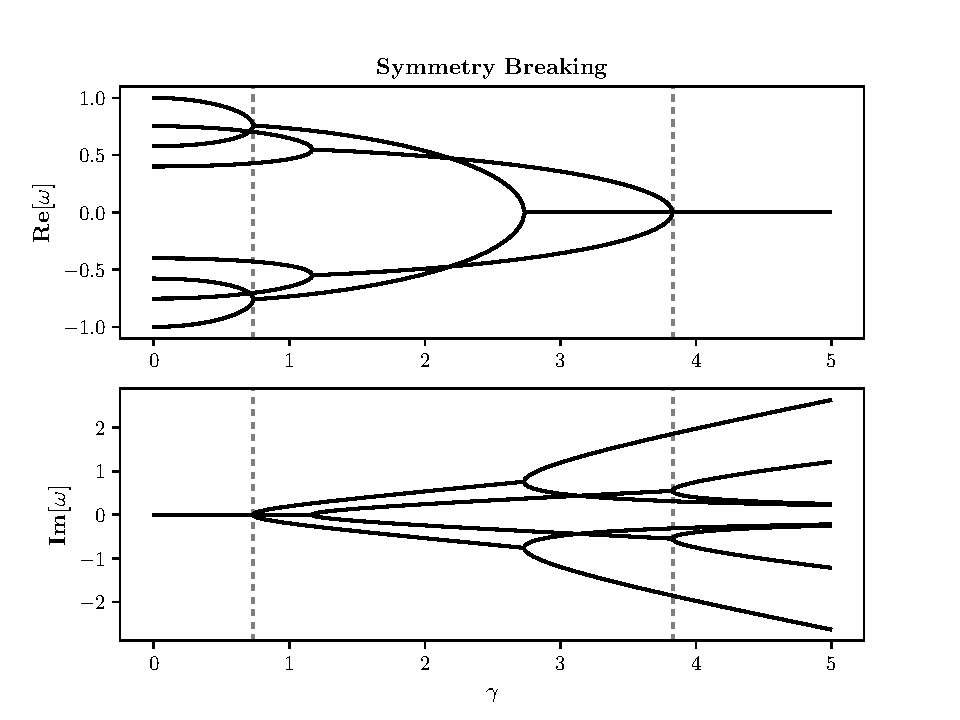
\includegraphics[scale=0.8]{pt_breaking.pdf}
	\caption{Graph for n=2 with $\kappa = 1$ and $\kappa' = 2$}
\end{figure}

With this graph we can tell that there are four major points of splitting, but the most important ones, where normal modes are either entirely real or entirely complex, can be found at $\gamma \approx 0.73$ and $\gamma \approx 3.83$.

Currently, we are attempting to find more values of $\lambda'$ for larger and larger $n$ to attempt to find a pattern and determine $\lambda'$ from $n$. This would be invaluable in finding all normal modes of the circuit for arbitrary $n$, as well as taking the limit as $n \to \infty$. Additionally, we are in the process of obtaining the necessary materials to create this circuit and test it. I have also written a numerical solver for the eigenvalues for use when testing, and can use this to compare with Fatemeh's results.
\\
\\
\\
Thank you for your time.

\end{document}
